\documentclass[10pt,a4paper]{scrreprt}

\usepackage[margin=1.9cm,top=2cm,bottom=2.2cm]{geometry}
\usepackage[table]{xcolor}
\usepackage{colortbl}
\usepackage{booktabs}
\usepackage{array}
\usepackage{enumitem}
\usepackage{tcolorbox}
\tcbuselibrary{skins}
\usepackage{tikz}
\usetikzlibrary{positioning,calc}
\usepackage{fontawesome5}
\usepackage{multicol}
\usepackage{fancyhdr}
\usepackage{lastpage}
\usepackage{ragged2e}

% ---------- palette ----------
\definecolor{leasenavy}{RGB}{26,41,62}
\definecolor{leasegold}{RGB}{170,138,86}
\definecolor{leaseslate}{RGB}{99,108,120}
\definecolor{leasepaper}{RGB}{246,244,239}
\definecolor{leaseline}{RGB}{213,208,196}

\pagestyle{fancy}
\fancyhf{}
\renewcommand{\headrulewidth}{0.6pt}
\renewcommand{\headrule}{\hbox to\headwidth{\color{leaseline}\leaders\hrule height \headrulewidth\hfill}}
\fancyhead[L]{\small\color{leaseslate} Commercial Lease Agreement}
\fancyhead[R]{\small\color{leaseslate} Nexa Tower \textbullet\ Suite 400}
\fancyfoot[C]{\small\color{leaseslate} Page \thepage\ of \pageref{LastPage}}
\renewcommand{\footrulewidth}{0.4pt}
\renewcommand{\footrule}{\hbox to\headwidth{\color{leaseline}\leaders\hrule height \footrulewidth\hfill}}

\setlength{\parindent}{0pt}
\setlength{\parskip}{2pt}
\setlength{\headheight}{22pt}

% ---------- article / clause machinery ----------
\newcounter{artcnt}
\newcounter{clausecnt}[artcnt]

\newcommand{\leasearticle}[1]{%
  \stepcounter{artcnt}%
  \setcounter{clausecnt}{0}%
  \vspace{4pt}%
  \noindent\begin{tcolorbox}[colback=leasenavy,colframe=leasenavy,boxrule=0pt,arc=0pt,
    left=10pt,right=10pt,top=4pt,bottom=4pt,before skip=0pt,after skip=0pt]
    {\color{white}\large\bfseries ARTICLE \arabic{artcnt}\quad #1}
  \end{tcolorbox}
  \vspace{3pt}%
}

\newcommand{\leaseclause}[1]{%
  \stepcounter{clausecnt}%
  \vspace{2pt}\noindent{\bfseries\color{leasenavy}\arabic{artcnt}.\arabic{clausecnt}\quad #1}\par\vspace{1pt}%
}

\newcommand{\exhibitheading}[2]{%
  \vspace{8pt}%
  \noindent\begin{tcolorbox}[colback=leasepaper,colframe=leasenavy,boxrule=1pt,arc=0pt,
    left=12pt,right=12pt,top=5pt,bottom=5pt,before skip=0pt,after skip=0pt]
    {\color{leasegold}\bfseries EXHIBIT #1}\\[1pt]
    {\color{leasenavy}\LARGE\bfseries #2}
  \end{tcolorbox}
  \vspace{4pt}%
}

\newcommand{\factrow}[3]{%
  \noindent{\color{leasegold}#1}\ \ {\bfseries\color{leasenavy}#2:}\ \ #3\par\smallskip%
}

\begin{document}

% ============================================================= %
% COVER / TITLE BLOCK
% ============================================================= %
\thispagestyle{fancy}

\begin{center}
  {\color{leasegold}\rule{4cm}{1.2pt}}\\[6pt]
  {\Large\color{leaseslate} COMMERCIAL LEASE AGREEMENT}\\[2pt]
  {\huge\bfseries\color{leasenavy} Nexa Tower --- Suite 400}\\[6pt]
  {\color{leaseslate} 1200 Founders Parkway, Riverton, NY 10940}\\[4pt]
  {\color{leasegold}\rule{4cm}{1.2pt}}
\end{center}

\vspace{5pt}

\noindent\begin{tcolorbox}[colback=leasepaper,colframe=leaseline,boxrule=0.8pt,arc=2pt,
  left=12pt,right=12pt,top=10pt,bottom=10pt]
\begin{minipage}[t]{0.48\textwidth}
  \factrow{\faBuilding}{Landlord}{Meridian Property Holdings, LLC}
  \factrow{\faUsers}{Tenant}{Synapse Analytics, Inc.}
  \factrow{\faMapMarker}{Premises}{Suite 400, approx.\ 8{,}450 RSF}
\end{minipage}\hfill
\begin{minipage}[t]{0.48\textwidth}
  \factrow{\faCalendar}{Lease Term}{84 months (7 years)}
  \factrow{\faClock}{Commencement}{September 1, 2026}
  \factrow{\faDollarSign}{Year 1 Base Rent}{\$291{,}525.00 per annum}
\end{minipage}
\end{tcolorbox}

\vspace{6pt}

This Commercial Lease Agreement (this ``\textbf{Lease}'') is made and entered into as of
\textbf{August 4, 2026} (the ``\textbf{Effective Date}''), by and between
\textbf{Meridian Property Holdings, LLC}, a Delaware limited liability company
(``\textbf{Landlord}''), and \textbf{Synapse Analytics, Inc.}, a Delaware corporation
(``\textbf{Tenant}''). Landlord and Tenant are referred to individually as a ``Party'' and
collectively as the ``Parties.''

\textbf{RECITALS}

\textbf{WHEREAS}, Landlord is the owner of that certain office building known as Nexa Tower,
located at 1200 Founders Parkway, Riverton, NY 10940 (the ``\textbf{Building}''), situated on
the parcel of land more particularly described in \textbf{Exhibit A} attached hereto (together
with the Building, the ``\textbf{Property}'');

\textbf{WHEREAS}, Tenant desires to lease from Landlord, and Landlord desires to lease to
Tenant, that certain premises consisting of approximately 8{,}450 rentable square feet located
on the fourth (4th) floor of the Building and identified as Suite 400 (the ``\textbf{Premises}''),
as depicted on the floor plan attached hereto as \textbf{Exhibit A-1}; and

\textbf{WHEREAS}, the Parties desire to set forth their respective rights and obligations with
respect to the Premises on the terms and conditions set forth below;

\textbf{NOW, THEREFORE}, in consideration of the mutual covenants contained herein and other
good and valuable consideration, the receipt and sufficiency of which are hereby acknowledged,
the Parties agree as follows.

% ============================================================= %
\leasearticle{Premises and Term}

\leaseclause{Demised Premises}
Landlord hereby leases to Tenant, and Tenant hereby leases from Landlord, the Premises, together
with the non-exclusive right to use, in common with other tenants of the Building, the Common
Areas (as defined in Section 1.3), subject to the terms of this Lease.

\leaseclause{Lease Term}
The term of this Lease (the ``\textbf{Term}'') shall commence on September 1, 2026 (the
``\textbf{Commencement Date}'') and, unless sooner terminated as provided herein, shall expire
on August 31, 2033 (the ``\textbf{Expiration Date}''), constituting a Term of eighty-four (84)
full calendar months.

\leaseclause{Common Areas}
``Common Areas'' means all areas of the Property designated by Landlord from time to time for
the general non-exclusive use of tenants, including lobbies, corridors, elevators, restrooms on
multi-tenant floors, loading areas, and the parking facility described in Section 9.2.

\leaseclause{Renewal Options}
Provided Tenant is not then in monetary or material non-monetary default, Tenant shall have two
(2) successive options to renew this Lease for additional periods of five (5) years each, at
ninety-five percent (95\%) of then-prevailing fair market rent, exercisable by written notice to
Landlord not less than nine (9) months prior to the expiration of the then-current Term.

% ============================================================= %
\leasearticle{Rent and Additional Rent}

\leaseclause{Base Rent}
Tenant shall pay Landlord, without notice, demand, deduction, or offset, the annual base rent
(``\textbf{Base Rent}'') set forth below, in equal monthly installments payable in advance on or
before the first day of each calendar month during the Term.

\begin{center}
\renewcommand{\arraystretch}{1.0}
\begin{tabular}{lrrr}
\toprule
\rowcolor{leasenavy}
{\color{white}\textbf{Lease Year}} & {\color{white}\textbf{Rate / RSF}} &
{\color{white}\textbf{Annual Base Rent}} & {\color{white}\textbf{Monthly Installment}}\\
\midrule
Year 1 (2026--2027) & \$34.50 & \$291{,}525.00 & \$24{,}293.75\\
Year 2 (2027--2028) & \$35.54 & \$300{,}270.75 & \$25{,}022.56\\
Year 3 (2028--2029) & \$36.60 & \$309{,}278.87 & \$25{,}773.24\\
Year 4 (2029--2030) & \$37.70 & \$318{,}557.24 & \$26{,}546.44\\
Year 5 (2030--2031) & \$38.83 & \$328{,}113.95 & \$27{,}342.83\\
Year 6 (2031--2032) & \$39.99 & \$337{,}957.37 & \$28{,}163.11\\
Year 7 (2032--2033) & \$41.19 & \$348{,}096.09 & \$29{,}008.01\\
\bottomrule
\end{tabular}
\end{center}

\leaseclause{Additional Rent -- Operating Expenses}
In addition to Base Rent, Tenant shall pay its proportionate share (7.4\%) of the Property's
Operating Expenses, currently estimated at \$9.25 per RSF per annum (\$78{,}162.50 annually, or
\$6{,}513.54 monthly), subject to annual reconciliation within ninety (90) days following each
calendar year-end. ``Operating Expenses'' includes, without limitation, common area maintenance,
property insurance, property taxes, and management fees, but excludes capital improvements not
required by Applicable Law.

\leaseclause{Late Charges}
Any Base Rent or Additional Rent not received within five (5) business days of its due date
shall accrue a late charge equal to five percent (5\%) of the overdue amount, plus interest at
the lesser of twelve percent (12\%) per annum or the maximum rate permitted by law.

\leaseclause{Net Lease}
This Lease is intended to be a triple-net (NNN) lease. Except as expressly set forth herein,
Landlord shall receive Base Rent free of any deduction, offset, or charge of any kind.

% ============================================================= %
\leasearticle{Security Deposit}

\leaseclause{Amount and Purpose}
Upon execution of this Lease, Tenant shall deposit with Landlord the sum of \textbf{\$48{,}587.50}
(the ``\textbf{Security Deposit}''), equal to two (2) months of Year 1 Base Rent, as security for
the faithful performance of Tenant's obligations hereunder.

\leaseclause{Application and Return}
Landlord may apply all or part of the Security Deposit to cure any default by Tenant, in which
case Tenant shall restore the deposit to its original amount within ten (10) business days of
written demand. Provided Tenant has fully performed its obligations, Landlord shall return any
unapplied balance within forty-five (45) days after the later of the Expiration Date or Tenant's
surrender of the Premises.

% ============================================================= %
\leasearticle{Use of Premises}

\leaseclause{Permitted Use}
Tenant shall use the Premises solely for general office purposes, data analytics operations, and
software research and development, and for no other purpose without Landlord's prior written
consent, which shall not be unreasonably withheld.

\leaseclause{Compliance with Law}
Tenant shall, at its sole cost, comply with all Applicable Laws relating to its specific use and
occupancy of the Premises, including the Americans with Disabilities Act with respect to
Tenant's alterations and business operations.

\leaseclause{Prohibited Uses}
Tenant shall not use the Premises in any manner that (a) violates any Applicable Law, (b)
constitutes a nuisance or waste, (c) increases the Building's insurance premiums, or (d)
interferes with the quiet enjoyment of other tenants.

% ============================================================= %
\leasearticle{Maintenance, Repairs, and Alterations}

\leaseclause{Landlord's Obligations}
Landlord shall maintain and repair, in good working order, the Building structure, roof,
foundation, exterior walls, Common Areas, and the base-building mechanical, electrical, plumbing,
and HVAC systems serving the Premises, the cost of which is included in Operating Expenses.

\leaseclause{Tenant's Obligations}
Tenant shall, at its sole cost, maintain the interior, non-structural portions of the Premises,
including fixtures, doors, floor coverings, and any supplemental equipment installed by Tenant,
in good condition, ordinary wear and tear excepted.

\leaseclause{Alterations}
Tenant shall not make any alterations, additions, or improvements to the Premises exceeding
\$25{,}000 in any single instance without Landlord's prior written consent. All approved
alterations shall become part of the Premises and, unless Landlord directs otherwise in writing
at the time of approval, shall remain upon expiration of the Term.

% ============================================================= %
\leasearticle{Insurance and Indemnification}

\leaseclause{Tenant's Insurance}
Tenant shall maintain, at its sole expense, throughout the Term: (a) commercial general
liability insurance with limits of not less than \$2{,}000{,}000 per occurrence; (b) property
insurance covering Tenant's personal property and improvements on a full replacement cost basis;
and (c) workers' compensation insurance as required by Applicable Law. Landlord shall be named
as an additional insured on Tenant's liability policy.

\leaseclause{Waiver of Subrogation}
Each Party waives, and shall cause its insurers to waive, any right of subrogation against the
other Party for losses covered by property insurance carried pursuant to this Lease.

\leaseclause{Mutual Indemnification}
Tenant shall indemnify, defend, and hold harmless Landlord from claims arising from Tenant's use
of the Premises or breach of this Lease, except to the extent caused by Landlord's negligence or
willful misconduct, and Landlord shall indemnify Tenant on a reciprocal basis.

% ============================================================= %
\leasearticle{Assignment and Subletting}

\leaseclause{Consent Required}
Tenant shall not assign this Lease or sublet all or any portion of the Premises without
Landlord's prior written consent, which shall not be unreasonably withheld, conditioned, or
delayed, provided the proposed assignee or subtenant is creditworthy and its intended use is
consistent with Article 4.

\leaseclause{Permitted Transfers}
Notwithstanding Section 7.1, Tenant may assign this Lease or sublet the Premises without
Landlord's consent to any entity controlling, controlled by, or under common control with
Tenant, or to a successor entity resulting from merger, acquisition, or sale of substantially all
of Tenant's assets, provided Landlord receives ten (10) days' prior written notice.

% ============================================================= %
\leasearticle{Default and Remedies}

\leaseclause{Events of Default}
Each of the following constitutes an ``\textbf{Event of Default}'': (a) failure to pay Rent within
five (5) business days after written notice of non-payment; (b) failure to perform any other
obligation under this Lease within thirty (30) days after written notice, or such longer period
as reasonably required to cure a non-monetary default commenced promptly and pursued diligently;
and (c) Tenant's bankruptcy, insolvency, or assignment for the benefit of creditors.

\leaseclause{Landlord's Remedies}
Upon an uncured Event of Default, Landlord may, without prejudice to any other remedy: (a)
terminate this Lease and recover all damages permitted by law, including the present value of
the remaining Rent; (b) terminate Tenant's right of possession without terminating this Lease
and relet the Premises on Tenant's account; or (c) pursue any other remedy available at law or
in equity.

\leaseclause{Landlord Default}
If Landlord fails to perform any material obligation under this Lease within thirty (30) days
after written notice from Tenant (or such longer period as reasonably required), Tenant may
pursue all remedies available at law or in equity, including, if Landlord's failure materially
and adversely affects Tenant's use of the Premises, a proportionate abatement of Rent.

% ============================================================= %
\leasearticle{Signage, Parking, and Access}

\leaseclause{Building-Standard Signage}
Tenant shall be entitled, at Landlord's building-standard specifications and at Tenant's cost,
to (a) one identification listing on the Building lobby directory and (b) suite entry signage,
subject to Landlord's prior written approval of design and placement.

\leaseclause{Parking}
Landlord shall make available to Tenant twenty-one (21) unreserved parking spaces in the
Building's parking facility at no additional charge during the Term, in accordance with the
Rules and Regulations attached as \textbf{Exhibit B}.

\leaseclause{Access}
Tenant shall have access to the Premises twenty-four (24) hours per day, seven (7) days per
week, subject to reasonable security procedures and any temporary restrictions required for
Building repairs, emergencies, or as required by Applicable Law.

% ============================================================= %
\leasearticle{Notices and Miscellaneous}

\leaseclause{Notices}
All notices under this Lease shall be in writing and delivered by nationally recognized courier
or certified mail, return receipt requested, to the addresses below, or such other address as a
Party designates by notice given in accordance herewith.

\noindent\color{leaseline}\rule{\linewidth}{0.6pt}\color{black}\\[2pt]
\noindent\begin{minipage}[t]{0.48\textwidth}
\textbf{If to Landlord:}\\
Meridian Property Holdings, LLC\\
500 Apex Plaza, Suite 1100\\
Riverton, NY 10940\\
Attn: Asset Management
\end{minipage}\hfill
\begin{minipage}[t]{0.48\textwidth}
\textbf{If to Tenant:}\\
Synapse Analytics, Inc.\\
1200 Founders Parkway, Suite 400\\
Riverton, NY 10940\\
Attn: General Counsel
\end{minipage}
\par\vspace{2pt}
\noindent\color{leaseline}\rule{\linewidth}{0.6pt}\color{black}

\leaseclause{Governing Law}
This Lease shall be governed by and construed in accordance with the laws of the State of New
York, without regard to its conflict-of-laws principles.

\leaseclause{Entire Agreement}
This Lease, together with Exhibits A and B attached hereto, constitutes the entire agreement
between the Parties with respect to its subject matter and supersedes all prior negotiations,
representations, and agreements, whether written or oral.

\leaseclause{Amendments}
No amendment or modification of this Lease shall be effective unless in writing and signed by
both Parties.

\leaseclause{Severability}
If any provision of this Lease is held invalid or unenforceable, the remainder shall continue in
full force and effect.

\vspace{8pt}
\textbf{IN WITNESS WHEREOF}, the Parties have executed this Lease as of the Effective Date first
written above.

\vspace{5pt}
\noindent\begin{minipage}[t]{0.46\textwidth}
\textbf{LANDLORD:}\\[2pt]
Meridian Property Holdings, LLC\\[22pt]
\color{leaseline}\rule{0.9\linewidth}{0.8pt}\\[2pt]
\color{black}By: Daniel Whitfield\\
Title: Authorized Signatory\\
Date: \makebox[3cm]{\hrulefill}
\end{minipage}\hfill
\begin{minipage}[t]{0.46\textwidth}
\textbf{TENANT:}\\[2pt]
Synapse Analytics, Inc.\\[22pt]
\color{leaseline}\rule{0.9\linewidth}{0.8pt}\\[2pt]
\color{black}By: Priya Shenoy\\
Title: Chief Executive Officer\\
Date: \makebox[3cm]{\hrulefill}
\end{minipage}
\par

% ============================================================= %
% EXHIBIT A
% ============================================================= %
\exhibitheading{A}{Legal Description \& Premises Depiction}

\textbf{Legal Description of the Property.} All that certain parcel of land situated in the City
of Riverton, County of Delford, State of New York, together with all improvements thereon,
known as Nexa Tower, and more particularly described as Lot 14, Block 6, of the Founders
Parkway Commercial Subdivision, as recorded in the Delford County land records, comprising
approximately 1.87 acres.

\textbf{Exhibit A-1 -- Approximate Floor Plan of Suite 400 (Not to Scale)}

\vspace{-4pt}
\begin{center}
\begin{tikzpicture}[scale=0.62, every node/.style={font=\small,align=center}]
\draw[thick,leasenavy,fill=leasepaper] (0,0) rectangle (10,6);
\draw[leaseslate] (0,4.5) rectangle (3,6);
\node at (1.5,5.25) {Reception};
\draw[leaseslate] (3,1.5) rectangle (10,6);
\node at (6.5,3.75) {Open Workspace};
\draw[leaseslate] (0,2.5) rectangle (3,4.5);
\node at (1.5,3.5) {Conference\\Room};
\draw[leaseslate] (0,1) rectangle (3,2.5);
\node at (1.5,1.75) {Server /\\Data Room};
\draw[leaseslate] (0,0) rectangle (3,1);
\node at (1.5,0.5) {Break Room};
\draw[leaseslate] (3,0) rectangle (10,1.5);
\node at (6.5,0.75) {Private Offices (6)};
\draw[leasegold,thick] (3,0) -- (3,6);
\draw[leaseslate,->] (5,-0.75) -- (5,-0.25);
\node[leaseslate,font=\scriptsize] at (5,-0.95) {N};
\end{tikzpicture}
\end{center}

\vspace{-6pt}
\begin{center}
\small\color{leaseslate} Figure A-1: Suite 400, Fourth Floor, Nexa Tower --- approximately
8{,}450 rentable square feet.
\end{center}

% ============================================================= %
% EXHIBIT B
% ============================================================= %
\exhibitheading{B}{Building Rules and Regulations}

The following rules and regulations are attached to and made a part of the Lease. In the event
of any conflict between this Exhibit B and the body of the Lease, the terms of the Lease shall
control.

\begin{multicols}{2}
\begin{enumerate}[leftmargin=*,itemsep=2pt,label=\arabic*.]
\item The sidewalks, entrances, halls, and stairways of the Building shall not be obstructed by
  any tenant or used for any purpose other than ingress and egress.
\item No tenant shall place any signage, advertisement, or notice visible from outside the
  Premises without Landlord's prior written approval.
\item Deliveries and freight movement shall be made only through the loading dock and freight
  elevator, and only between 7:00 a.m. and 6:00 p.m. on business days unless otherwise approved.
\item No cooking odors, food preparation fumes, or similar emissions shall be permitted to
  escape the Premises into Common Areas or adjoining premises.
\item Tenant shall not install supplemental HVAC, plumbing, or electrical equipment without
  Landlord's prior written consent and compliance with Building engineering standards.
\item After-hours HVAC service requested by Tenant shall be billed at Landlord's then-current
  hourly rate, currently \$65.00 per hour per zone.
\item No animals of any kind shall be brought into or kept in the Building, except service
  animals as required by Applicable Law.
\item Smoking is prohibited within the Building and within twenty-five (25) feet of all
  Building entrances.
\item Bicycles may be stored only in the designated ground-floor bicycle room and shall not be
  brought into elevators, lobbies, or the Premises.
\item Tenant shall dispose of ordinary trash in designated receptacles; bulk or hazardous waste
  requires prior coordination with the property manager.
\item Canvassing, soliciting, and peddling in the Building are prohibited, and tenants shall
  report any such activity to the property manager.
\item Tenant shall not overload floors, electrical circuits, or elevators beyond posted capacity
  limits, and shall not change Premises locks without providing Landlord a duplicate key.
\end{enumerate}
\end{multicols}

\vspace{5pt}
\noindent\begin{tcolorbox}[colback=leasepaper,colframe=leasegold,boxrule=0.8pt,arc=1pt,
  left=10pt,right=10pt,top=6pt,bottom=6pt]
\small\faExclamationTriangle\ \ \textbf{Landlord reserves the right} to amend, waive, or
supplement these Rules and Regulations from time to time upon reasonable written notice,
provided such changes are applied uniformly to all tenants of the Building and do not materially
increase Tenant's obligations under the Lease.
\end{tcolorbox}

\end{document}
